\providecommand{\main}{../..}
\documentclass[../../main.tex]{subfiles}

\begin{document}

\lesson{20}{23/04/20}

We have shown that, in the absence of spin-spin interactions, the Ising Model does not predict any phase transition. %Ease the connection with previous lecture

\medskip

So, let's study the \textbf{interacting case} $J\neq 0$ in one dimension $d=1$. In this case, the volume $V$, which coincides with the number of cells (as we have fixed the lattice step $a$ to $1$ with a choice of units), is more properly a length $L \equiv V$.

\medskip

For simplicity, we start from the case of \textbf{no external field} $b=0$ and \textbf{open boundary conditions} (fig. \ref{fig:obcd1}).   

\begin{figure}[H]
    \centering
    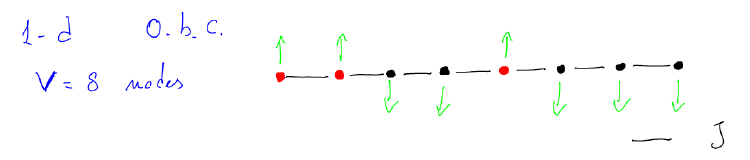
\includegraphics[width=0.7\textwidth]{\main/Images/image016.png}
    \caption{One-dimensional Ising Model with \textbf{open} boundary conditions.\label{fig:obcd1}}
\end{figure}

The partition function is given by:
\begin{align*}
    Z_L(K) &\underset{(\ref{eqn:Z-Is})}{=} 
    \sum_{\{\bm{\sigma}\}}\exp\left( K \sum_{\langle x,y \rangle} \sigma_x \sigma_y \right) =
    \sum_{\sigma_1 = \pm 1} \cdots \sum_{\sigma_{L-1}=\pm 1} \hlc{Yellow}{\sum_{\sigma_L = \pm 1}} e^{K \sigma_1 \sigma_2} e^{K \sigma_2 \sigma_3} \cdots \hlc{Yellow}{e^{K \sigma_{L-1} \sigma_L}} =\\
    &\underset{(a)}{=}  \sum_{\sigma_1 = \pm 1} \cdots \sum_{\sigma_{L-1}=\pm 1} e^{K \sigma_1 \sigma_2} \cdots e^{K \sigma_{L-2} \sigma_{L-1}} 2 \cosh (K \sigma_{L-1})
\end{align*}
where in (a) we summed over the last spin $\sigma_L$. Note that $\cosh$ is even, and so (thanks to our choice of \textit{symmetric} spin-like variables):
\begin{align*}
   2\cosh(K \sigma_{L-1}) = 2 \cosh(\pm K)  = 2 \cosh(K)
\end{align*}
and so:
\begin{align*}
    Z_L(K) &= 2\cosh K  \underbrace{\sum_{\sigma_1 = \pm 1} \cdots \sum_{\sigma_{L-1}=\pm 1} e^{K \sigma_1 \sigma_2} \cdots e^{K \sigma_{L-2} \sigma_{L-1}} }_{Z_{L-1}(K)}  = 2\cosh (K) Z_{L-1}(K)
\end{align*}
Reiterating:
\begin{align*}
    Z_L(K) = (2\cosh K)^L \underset{(\ref{eqn:Z-Is})}{\equiv}  e^{- \beta L f(K)} 
\end{align*}
Taking the logarithm of both sides:
\begin{align*}
    L \ln (2 \cosh K) = -\beta L f(K) \Rightarrow -\beta f(K) = \ln(2\cosh K)
\end{align*}

\begin{figure}[H]
    \centering
    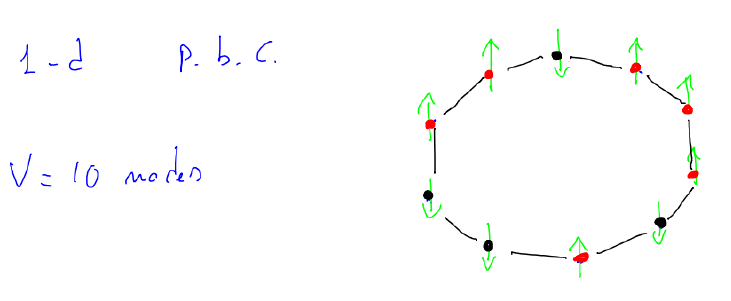
\includegraphics[width=0.7\textwidth]{\main/Images/image017.png}
    \caption{One-dimensional Ising Model with \textbf{periodic} boundary conditions.\label{fig:pbcd1}}
\end{figure}

If we had chosen \textbf{periodic boundary conditions} instead (fig. \ref{fig:pbcd1}) and $h\neq 0$, the partition function would have been:
\begin{align}\label{eqn:Zp}
    Z &\underset{(\ref{eqn:Z-Is})}{=}  \sum_{\{\bm{\sigma}\}} \exp\left(K \sum_{\langle x,y \rangle} \sigma_x \sigma_y + h \sum_x \sigma_x\right)  =\\
    &= \sum_{\sigma_1 \pm 1} \cdots \sum_{\sigma_L = \pm 1} e^{K \sigma_1 \sigma_2} \cdots e^{K \sigma_{L-1} \sigma_L} \hlc{Yellow}{e^{K \sigma_{L} \sigma_{1}} }e^{h \sigma_1} \cdots e^{h \sigma_L}
\end{align} 
Note how the last spin $\sigma_L$ interacts with the first one $\sigma_1$. We can rewrite the spin-spin interactions more compactly as:
\begin{align}\label{eqn:sus1}
    e^{K \sigma_1 \sigma_2} \cdots e^{K \sigma_{L-1} \sigma_L} e^{K \sigma_{L} \sigma_{1}} = \prod_{i=1}^L e^{K \sigma_i \sigma_{i+1}} \qquad \sigma_{L+1} \equiv \sigma_1
\end{align}
With a trick, we can rewrite also the terms $e^{h \sigma_i}$ as a product over \textit{pairs} $(\sigma_i, \sigma_{i+1})$. Thanks to p.b.c., each cell is \textit{connected} to exactly $2$ neighbouring cells (in $d=1$) and so a product over pairs contains the product of \textit{squares} of each node - because each cell is multiplied by itself once for every neighbour: 
\begin{align}\label{eqn:sus2}
    \prod_{i=1}^L e^{h \sigma_i} = \prod_{\langle i, j \rangle} \exp\left(h \frac{\sigma_i + \sigma_j}{2} \right) = \prod_{i=1}^L \exp\left(h \frac{\sigma_i + \sigma_{i+1}}{2} \right) \qquad \sigma_{L+1} \equiv \sigma_1
\end{align}
Substituting (\ref{eqn:sus1}) and (\ref{eqn:sus2}) back in (\ref{eqn:Zp}) leads to:
\begin{align} \label{eqn:Zp2}
    Z = \sum_{\{\bm{\sigma}\}} \prod_{i=1}^L \exp\left(K \sigma_i \sigma_{i+1} + h \frac{\sigma_i + \sigma_{i+1}}{2} \right)
\end{align}
Let's define a \textbf{matrix} \textbf{T}  with entries equal to the factors in (\ref{eqn:Zp2}):
\begin{align}\label{eqn:transfer-elements}
    T_{\sigma \sigma'} \equiv \exp\left(K \sigma \sigma' + h \frac{\sigma + \sigma'}{2} \right)
\end{align}
As $\sigma,\sigma' \in \{\pm 1\}$, \textbf{T} is a $2 \times 2$ matrix:
\begin{align*}
    \textbf{T}  = \begin{blockarray}{l*{2}{c}}
        \begin{block}{l*{2}{>{\scriptstyle}c<{}}}
            & \sigma'=+1 & \sigma'=-1 \\
        \end{block}
        \begin{block}{>{\scriptstyle}r<{}(*{2}{c})}
            \sigma=+1 & e^{K+h} & e^{-K} \\
            \sigma=-1 & e^{-K}   & e^{K-h}\\
        \end{block}
    \end{blockarray}
\end{align*}
\textbf{T} is called the \textbf{transfer matrix} for the $d=1$ Ising Model with periodic boundaries. 

Substituting (\ref{eqn:transfer-elements}) in (\ref{eqn:Zp2}) leads to:
\begin{align*}
    Z &= \sum_{\{\bm{\sigma}\}} \prod_{i=1}^L T_{\sigma_i \sigma_{i+1}} = \sum_{\sigma_1 = \pm 1} \sum_{\sigma_2 = \pm 1} \cdots \sum_{\sigma_{L-1} = \pm 1} \sum_{\sigma_L = \pm 1} T_{\sigma_1 \sigma_2} T_{\sigma_2 \sigma_3} \cdots T_{\sigma_{L-1} \sigma_{L}} T_{\sigma_L \sigma_1} =\\
    &\underset{(a)}{=} 
    \sum_{\sigma_1 = \pm 1} (\underbrace{\textbf{T} \cdot \dots \cdot \textbf{T}}_{L \text{ times}})_{\sigma_1 \sigma_1} =
    \sum_{\sigma_1 = \pm 1} (\textbf{T}^L)_{\sigma_1 \sigma_1} = \operatorname{Tr} \textbf{T}^L 
\end{align*}
In (a), note that all the sums except the first one lead to a \textit{chain} of matrix multiplications:
\begin{align*}
    \sum_a A_{ia} B_{aj} = C_{ij}
\end{align*} 
So, at the end, $Z$ is the sum of the diagonal elements of $\textbf{T}^L$, i.e. its \textbf{trace}.

\medskip

\textbf{T} is symmetric, and so it is diagonalizable, and its eigenvalues are \textbf{real} numbers. Moreover, the trace is basis independent, and so we may compute it in the basis where \textbf{T} is diagonal. Let \textbf{P} be the invertible matrix needed for diagonalizing \textbf{T}, then \textbf{P T P$^{-1}$} $= \operatorname{diag}(\lambda_1, \lambda_2)$, where $\lambda_1$ and $\lambda_2$ are the \textit{eigenvalues} of \textbf{T}. Raising both sides to the $L$-th power, we get:
\begin{align*}
    (\textbf{P}\, \textbf{T}\,\textbf{P}^{-1})^L  = \textbf{P}\,\textbf{T}\,\cancel{\textbf{P}^{-1} \textbf{P}}\,\textbf{T}\,\cancel{\textbf{P}^{-1} \textbf{P}}\cdots \textbf{T}\, \textbf{P}^{-1} = \textbf{P}\,\textbf{T}^L\, \textbf{P}^{-1} = \left(\begin{array}{cc}
    \lambda_1^L & 0 \\ 
    0 & \lambda_2^L
    \end{array}\right)           
\end{align*} 
Then:
\begin{align*}
    \operatorname{Tr}(\textbf{P}\,\textbf{T}^L\,\textbf{P}^{-1}) = \operatorname{Tr}(\textbf{P}^{-1}\,\textbf{P}\,\textbf{T}^L) = \operatorname{Tr}(\textbf{T}^L) =\operatorname{Tr} \left(\begin{array}{cc}
    \lambda_1^L & 0 \\ 
    0 & \lambda_2^L
    \end{array}\right) = \lambda_1^L + \lambda_2^L
\end{align*}
And so:
\begin{align*}
    Z = \operatorname{Tr} \textbf{T}^L = \lambda_1^L + \lambda_2^L  \underset{(\ref{eqn:Z-Is})}{\equiv}  e^{-\beta L f(K,h)}
\end{align*}
Taking the logarithm of both sides:
\begin{align*}
    \ln Z = - \beta L f(K,h) = \ln (\lambda_1^L + \lambda_2^L)
\end{align*}
and dividing by $L$:
\begin{align*}
    \frac{\ln Z}{L} = - \beta f(K,h) = \frac{1}{L} \ln(\lambda_1^L + \lambda_2^L)  
\end{align*}
Suppose (without loss of generality) that $\lambda_1 < \lambda_2$. Then:
\begin{align*}
    -\beta f(K,h) = \frac{1}{L} \ln(\lambda_2^L \Big[1+\left(\frac{\lambda_1}{\lambda_2}\right)^L \Big]) = \frac{1}{\cancel{L}} \cancel{L} \ln \lambda_2 + \frac{1}{L} \ln \left[1+\left(\frac{\lambda_1}{\lambda_2}\right)^L \right]  
\end{align*}
In the thermodynamic limit $L \to \infty$, the larger eigenvalue $\lambda_2$ \textit{dominates}, and $(\lambda_1/\lambda_2)^L \to 0$, so that:
\begin{align}\label{eqn:f-limit}
    -\beta f(K,h) = \ln \lambda_2 + \frac{1}{L} \ln \left[1+\left(\frac{\lambda_1}{\lambda_2}\right)^L \right] \xrightarrow[L \to +\infty]{} \ln \lambda_2
\end{align} 

The eigenvalues can be computed (as usual) as the roots of the \textit{secular} (or \textit{characteristic}) equation:
\begin{align*}
    0 &= \operatorname{det}(\textbf{T} - \lambda \bb{I}) = \operatorname{det} \left|\begin{array}{cc}
    e^{K+h}-\lambda & e^{-K} \\ 
    e^{-K} & e^{K-h}-\lambda
    \end{array}\right| = (e^{K+h} -\lambda)(e^{K-h}-\lambda) - e^{-2K} =\\
    &= \lambda^2 -\lambda e^{K} \frac{e^h + e^{-h}}{\textcolor{Red}{2}}\textcolor{Red}{2} + \frac{e^{2K} - e^{-2K}}{\textcolor{Red}{2}}\textcolor{Red}{2} = \lambda^2 - \lambda e^K \cosh h + 2 \sinh 2K 
\end{align*} 
which are:
\begin{align*}
    \lambda_{1,2} &= e^K \cosh h \mp \sqrt{e^{2K} \cosh^2 h - 2 \sinh 2K} =\\
    &= e^K \cosh h \mp \sqrt{e^{2K} \sinh^2 h + e^{-2K}}
\end{align*}

The \textbf{magnetization} is given by:
\begin{align}\nonumber
    m &\underset{(\ref{eqn:magnetization})}{=}  -\pdv{h} (\beta f) \>\>\overset{\mathclap{L \to \infty}}{\underset{(\ref{eqn:f-limit})}{=}} \>\> \pdv{h} \ln \lambda_2 = \pdv{h} \ln (e^{K} \cosh h + \sqrt{e^{2K} \sinh^2 h + e^{-2K}}) =\\ \nonumber
    &= \frac{1}{e^{K} \cosh h + \sqrt{e^{2K} \sinh^2 h + e^{-2K}}} \left(e^{K} \sinh h + \frac{\cancel{2} e^{2K} \sinh h \cosh h}{\cancel{2} \sqrt{e^{2K} \sinh^2 h + e^{-2K}}} \right) =\\ \nonumber
    &= \frac{1}{e^{K} \cosh h + \sqrt{e^{2K} \sinh^2 h + e^{-2K}}} \frac{\textcolor{Red}{e^K} \sqrt{e^{2K} \sinh^2 h + e^{-2K}} + \textcolor{Red}{e}^{2\textcolor{Red}{K}} \cosh h}{\sqrt{\textcolor{Red}{e^{2K}} \sinh^2 h + \textcolor{Red}{e^{-2K}}}} =\\ \nonumber
    &\underset{(a)}{=}  \frac{1}{\bcancel{e^{K} \cosh h + \sqrt{e^{2K} \sinh^2 h + e^{-2K}}}} \frac{\bcancel{e^K \cosh h + \sqrt{e^{2K} \sinh^2 h + e^{-2K}}}}{\sqrt{\sinh^2 h + e^{-4K}}} =\\
    &=  \frac{\sinh h}{\sqrt{\sinh^2 h + e^{-4K}}} \underset{(b)}{=} \frac{\tanh h}{\sqrt{1 - \frac{1-e^{-4K}}{\cosh^2 h} }} \label{eqn:m-pbc}
\end{align}
where in (a) we divided numerator and denominator by $e^K$, and in (b) by $\cosh h$ and applied the identity $\cosh^2 h - \sinh^2 h = 1 \Rightarrow \sinh^2 h = \cosh^2 h - 1$. 

\medskip

Note that if $K = 0$, and so $J=0$ (non-interacting case), (\ref{eqn:m-pbc}) leads back to $m = \tanh h$, the result we already found in (\ref{eqn:mh}). Moreover, if $K > 0$ (ferromagnetic interaction), $m(K,h) > m(0,h)$ - meaning that spins align more easily to the external field if they can interact with their neighbours.

\medskip

Again, if $h=0$, $m(K,h=0) = 0$, and so the system is unable to magnetize in absence of an external field.

In fact, consider any average spin, e.g. $\langle \sigma_0 \rangle$:
\begin{align*}
    \langle \sigma_0 \rangle = \sum_{\{\bm{\sigma}\}} \exp\left(K \sum_{\langle x,y \rangle} \sigma_x \sigma_y\right)
\end{align*}
For any \textit{finite} system ($L < +\infty$) the sum over all states is a \textit{finite} sum, meaning that it evaluates to some finite number. Moreover, it is \textbf{odd} under the change of variables $\sigma_x \leftrightarrow \sigma_x' = -\sigma_x$:
\begin{align}\label{eqn:symmetry-arg}
    \langle \sigma_0 \rangle = \sum_{\{\bm{\sigma}\}} \exp\left(K \sum_{\langle x,y \rangle} \sigma_x \sigma_y\right)  \sigma_0 = -\sum_{\{\bm{\sigma}\}} \exp\left(K \sum_{\langle x,y \rangle} \sigma_x \sigma_y \right) \sigma_0 = -\langle \sigma_0 \rangle
\end{align} 
and so $\langle \sigma_0 \rangle = 0$. Clearly, this arguments holds for any spin (by translation invariance), and so in general $\langle \sigma_k \rangle = 0$ $\forall k$.

\section{Spontaneous magnetization}
To observe the rise of a \textbf{spontaneous magnetization} (which is the experimental result we wish to model), i.e. a non zero $m$ with no external field ($h=0$), we need to be careful in the \textit{order} of limits. In (\ref{eqn:symmetry-arg}) taking $h = 0$ first leads to $m = 0$ for any finite $V$ - and so also in the thermodynamic limit. The idea is then to \textit{exchange} the two limits:
\begin{align}\label{eqn:break1}
    m(T) = \lim_{h \to 0^+} \lim_{V \to+ \infty} \langle \sigma \rangle_{V,h}
\end{align}
So, first compute the magnetization $\langle \sigma \rangle$ for a finite volume $V$ and in presence of an external field $h \neq 0$. Then perform the thermodynamic limit $V \to \infty$, and only then let go the field $h \to 0^+$. The $m(T)$ so defined is the \textbf{spontaneous magnetization} of the system, and it can be non-zero.

\medskip

The idea is that the \textit{presence} of $h \neq 0$ \textit{breaks} the symmetry ($\bm{\sigma} \leftrightarrow -\bm{\sigma}$) of the system, invalidating argument (\ref{eqn:symmetry-arg}) and thus allowing a spontaneous magnetization.

\medskip

Equivalently, one can break the symmetry without using $h \neq 0$, but by imposing some \textit{fixed} boundary conditions, for example by setting all spins at the boundaries set to $+1$. In this case, the magnetization for a finite volume $V$ is denoted with $\langle \sigma \rangle_V^+$ (\textbf{plus} boundary condition). We can then take the thermodynamic limit:
\begin{align}\label{eqn:break2}
    m(T) = \lim_{V \to +\infty} \langle \sigma \rangle_V^+
\end{align}
The boundary effect will vanish when $V \to \infty$, but it will always break the symmetry of the Hamiltonian ($\bm{\sigma} \leftrightarrow -\bm{\sigma}$).

\medskip

Intuitively, (\ref{eqn:break1}) and (\ref{eqn:break2}) \textit{break} the symmetry in the \q{same direction} (the first with $h>0$, and the latter with $\sigma_i = +1$ at the boundaries), and so we expect them to lead to the same result at the end. For now, no instances in which (\ref{eqn:break1}) and (\ref{eqn:break2}) lead to different results are known.

\medskip

Clearly, we can also consider the limits \textit{from the other direction}, i.e. from $h < 0$, or with \textbf{down} boundary conditions ($\sigma_i = -1$ at the boundaries). The resulting magnetization will be the opposite:
\begin{align*}
    \lim_{h \downarrow 0^+} m(K,h) = \textcolor{Red}{-} \lim_{h \uparrow 0^-} m(K,h)
\end{align*} 

\label{par:no-phase-transition}
For the Ising Model in $d=1$, $m(T) = 0$. In fact, in computing $m$ in (\ref{eqn:m-pbc}) we first considered the thermodynamic limit $L \to \infty$ for the free energy (\ref{eqn:f-limit}) with $h \neq 0$. Then, taking $h \to 0$ (as already observed), leads to $m = 0$. So,\marginpar{No phase-transitions in $d=1$} unfortunately, the $d=1$ Ising Model \textbf{does not} suffice to capture the effect of spontaneous magnetization (and thus of a phase-transition), even when spin-spin interactions are considered. 

\medskip

To observe a phase-transition, we need to find where the free energy $f(K,h)$ is non-analytic. In general, it can be shown that $\forall d > 1$, and $\forall h \neq 0$, $f(K,h)$ is analytic everywhere. The only singular points happen at $h=0$ for $T < T_c$, where $T_c$ is called the \textbf{critical temperature}. 

\begin{figure}[H]
    \centering
    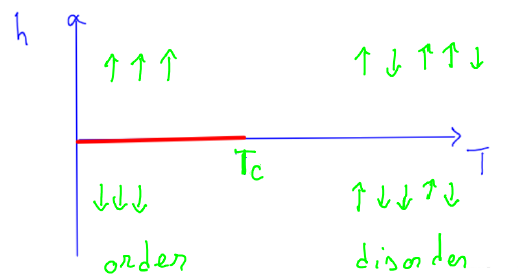
\includegraphics[width=0.7\textwidth]{\main/Images/image018.png} 
    \caption{Phase-diagram showing all parameters $(h,T)$ for which the Ising Model's free energy $f(K,h)$ is non-analytic, which lie on the red segment with $h=0$ and $T=(0,T_c]$. Taking the limit $h \to 0^\pm$ when $T < T_c$ will lead to a non-zero magnetization $m$ (positive if $h \downarrow 0^+$, negative if $h \uparrow 0^-$) - in other words the system \q{spontaneously {organizes}} in absence of an external field (\textbf{ordered phase}). The same limit when $T > T_c$ leads to $m = 0$ - here thermal fluctuations are too high, and the system remains in a random state (\textbf{disordered phase}).\label{fig:non-analytic}}
\end{figure}

\begin{figure}[H]
    \centering
    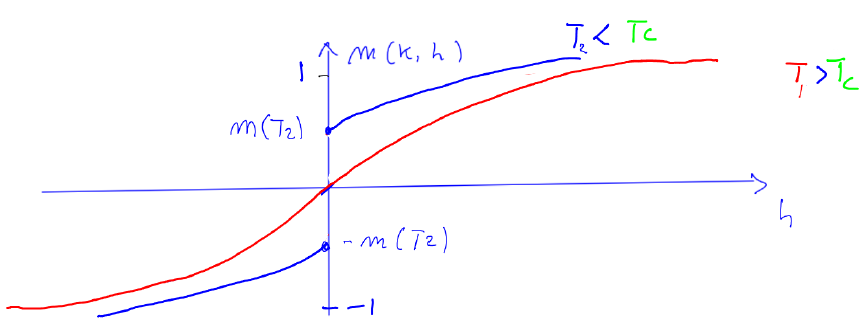
\includegraphics[width=0.7\textwidth]{\main/Images/image019.png}
    \caption{Magnetization at constant temperature $T$ as function of the field strength $h$ (i.e. along a \textit{vertical line} in fig. \ref{fig:m-critical}). If $T > T_c$, as for the red line, the result is the same we obtained in the non-interacting case (fig. \ref{fig:free-spin-m}), or the $d=1$ model. On the other hand, for $T < T_c$ (blue line), a singularity appears at $h=0$, with two possible limits for the magnetization.\label{fig:m-plot}}
\end{figure}

\begin{figure}[H]
    \centering
    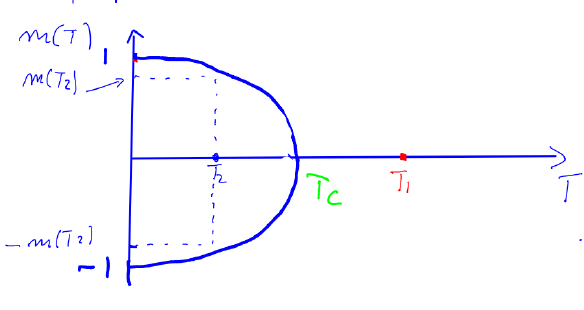
\includegraphics[width=0.7\textwidth]{\main/Images/image020.png}
    \caption{Bifurcation plot for the \textbf{spontaneous magnetization} $m(T)$, i.e. the intercept at $h=0$ of the curves in fig. \ref{fig:m-plot} at various temperatures. For $T > T_c$, all curves $m(h)$ cross the origin, and so lead to no spontaneous magnetization $m(T) = 0$. Conversely, for $T < T_c$, two opposite values of $m(T)$ are possible, depending on the taken limit $h \to 0^\pm$. Note that the region \q{inside the arc} is not reachable (\textbf{unphysical region}): for example at $T = T_2$ it is impossible to obtain a magnetization $|m| < |m(T_2)|$. \label{fig:spont-m}}
\end{figure}



\begin{figure}[H]
    \centering
    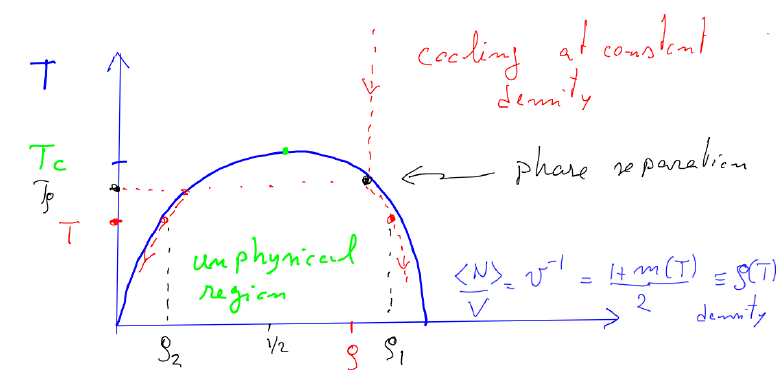
\includegraphics[width=0.7\textwidth]{\main/Images/image021.png}
    \caption{The analogue of the magnetization $m$ in the lattice gas is the \textbf{density} $\rho = v^{-1} = \langle N \rangle /V = (1+m(T))/2$. \label{fig:lattice-critical}} %TODO Mathematically derive the shift and rotation of that curve
\end{figure}

Consider the lattice gas model,\marginpar{\danger This part is still under revision!} with a fraction $\rho$ of occupied cells. Suppose we want to keep $\langle N \rangle$ fixed. This can be done by changing the chemical potential, which is the conjugate variable to $N$, and in the lattice gas model takes the role the external magnetic field had in the ferromagnetic Ising Model (in fact the magnetic field $b$ is a function of $\ln z$, which contains $\mu$).

Lowering the temperature (moving along the red dashed line), to keep $\rho$ fixed, $\mu$ has to change. When it reaches the blue curve, a \textit{phase separation} is observed, and the gas divides in two parts: one of low density $\rho_2$, and one with higher density $\rho_1$. Graphically, until the blue curve is reached, the gas is \q{well mixed}: every region has almost the same density. After, it is divided in mostly empty regions and very dense regions (fig. \ref{fig:fluid-sep}).

\begin{figure}[H]
    \centering
    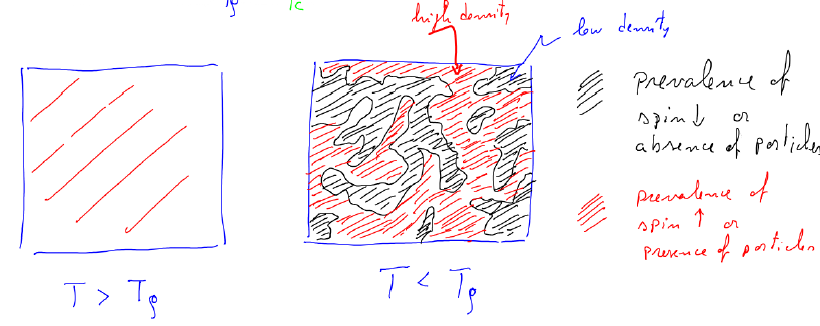
\includegraphics[width=0.7\textwidth]{\main/Images/image022.png}
    \caption{The lattice gas is well-mixed for $T > T_\rho$ (left figure), but separates in two phases with different densities for $T < T_\rho$.\label{fig:fluid-sep}}
\end{figure}

Let $f_i$ be the fraction of volume occupied by the fluid with density $\rho_i$ satisfies:
\begin{align*}
    f_1 \rho_1 + f_2 \rho_2 = \rho
\end{align*}
and $\rho$ is fixed and remains constant. Also $f_1 + f_2 = 1$. Then:
\begin{align*}
    \rho_1 = \frac{1+m(T)}{2}; \qquad \rho_2 = \frac{1-m(T)}{2}  
\end{align*}
leading to:
\begin{align*}
    f_1(T) = 1-f_2(T) = \frac{1}{2} \left(1+\frac{2 \rho -1}{m(T)} \right) 
\end{align*}

%Last 8 minutes
\begin{align*}
    \rho = \begin{cases}
        \frac{1+m(T_\rho)}{2} & \rho > \frac{1}{2}\\
        \frac{1-m(T_\rho)}{2} & \rho < \frac{1}{2}    
    \end{cases}
\end{align*}

$T_\rho$ is defined as the temperature at which the red dashed line intercepts the blue curve, i.e. at which phase separation occurs. 



\begin{figure}[H]
    \centering
    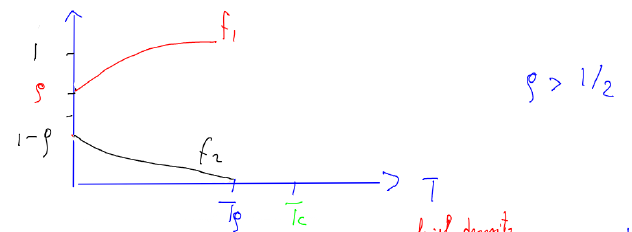
\includegraphics[width=0.7\textwidth]{\main/Images/image023.png}
    \caption{\label{fig:fluid-phases}}
\end{figure}

Spinoidal decomposition: try to enter in the unphysical region by rapidly cooling the gas. 
%TODO complete lattice gas analogy and results, explain spinoidal decomposition

\medskip

%Lecture 20 B
So we have found that the both the non-interacting case and the $d=1$ Ising Model do not present any kind of phase transition. To proceed, we need to considerate a higher dimensional case. One possible way is through numerical simulations, or by considering the exact solution of the $d=2$ case, for which the critical temperature turns out to be:
\begin{align*}
    T_c = \frac{2 \epsilon_0 / k_B}{\ln (1 + \sqrt{2})} 
\end{align*}
Often one considers the \textit{adimensional} critical parameter $k_c$, defined as:
\begin{align*}
    k_c \equiv \frac{\epsilon_0}{k_B T_c} = \frac{1}{2} \ln (1 + \sqrt{2}) = 0.44\dots  
\end{align*} 
which is such that $\sinh(2k_c) = 1$. %Motivate
For details see \cite{huang}. 

The specific heat at $b=0$ is:
\begin{align*}
    c_v(b=0, T) \underset{T \sim T_c}{\propto} - \ln \left|1-\frac{T}{T_c}  \right|
\end{align*}

The magnetization is $0$ above $T_c$, and for $T < T_c$ is given by:
\begin{align*}
    m(T) = \left[1-\frac{1}{\sinh^4(2K)} \right]^{1/8} \theta(T_c-T) \propto \theta(T_c - T) (T_c - T)^{1/8}
\end{align*}
The exponent $1/8$ is also called the $\beta$ exponent (not to be confused with $1/k_B T$). We will study this kind of \textit{power laws} for criticality in a later chapter. They are of particular importance because of their \textbf{universality} - i.e. very different systems sharing certain fundamental symmetries have the same behaviour when approaching $T_c$. (As anticipated, criticality is important to model complex systems). %TODO Complete Onsager's exact solution discussion, add references

\medskip

No rigorous \textit{exact} result is known for the case $h \neq 0$. 

\medskip

Another possibility to go on is to study low/high temperatures expansion of the Ising Model. 


\subsection{Low temperature expansion}
Consider the partition function for the Ising Model in $d$ dimensions:
\begin{align}\label{eqn:Z-again}
    Z= \sum_{\{\bm{\sigma}\}} \exp\left(K \sum_{\langle x,y \rangle} \sigma_x \sigma_y + h \sum_x \sigma_x\right) = e^{-\beta V f(K,h)} \qquad \substack{h = \beta b\\K = \beta J}
\end{align}
The idea is to \textit{approximate} $Z$ with a truncated sum, considering only the most \textit{relevant} states. Suppose $h\neq 0$ - for instance $h > 0$. Then, at very low temperature, we expect almost all spins to be aligned towards $h$. In this situation, the \textit{most probable} configurations $\bm{\sigma}$ comprehend the one where all spins are aligned ($\sigma_i \equiv +1$), followed by the ones where only a few spins are \textit{flipped}. Each of them \textit{refines} the value of $Z$ - and if a sufficient number of terms is considered, we can understand the low-temperature behaviour of the system.

\medskip

In general, however, it is not clear how to find the \textbf{radius of convergence} of such a series. In practice, the low-temperature approximation works well for $T \sim 0$, and breaks down when approaching $T_c$, where $Z$ is non-analytic.  

\medskip

So, let's start computing some terms. In the following we will assume for simplicity \textbf{periodic} boundary conditions, meaning that every cell has exactly $2d$ neighbours.


When no spins are flipped $\sigma_i \equiv +1$, the exponential becomes:
\begin{align}\label{eqn:term0a}
    \mathcal{N}_0 =\exp\Bigg(K \underbrace{\sum_{\langle x,y \rangle} 1 }_{A}+ h \underbrace{\sum_x 1}_{B}\Bigg) \underset{(\ref{eqn:sum2})}{=}  \exp\left(K V d + h V\right)
\end{align}  
Let's fix $d=2$ to allow some visualization. Then:
\begin{align}\label{eqn:term0}
    \mathcal{N}_0 = \exp[V(2K + h)]
\end{align}

\medskip

Suppose now we flip one spin $\sigma_i = -1$ (it does not matter which, as the system is transitionally invariant), and consider how much each of the two sums $A$ and $B$ in (\ref{eqn:term0a}) changes (fig. \ref{fig:one-flip}).

\begin{figure}[H]
    \centering
    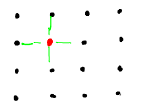
\includegraphics[width=0.3\textwidth]{\main/Images/image024.png}
    \caption{Square lattice with one flipped spin (in red). The affected interactions are represented by the green edges.\label{fig:one-flip}}
\end{figure}

$B$ is just the sum over spins. As $\sigma_i$ was $+1$ and now it is $-1$, the change $\Delta B$ is $-1 - (+1) = -2$, so $B = N \to N-2$.

On the other hand, changing one spin in $A$ affects all the pairs $(\sigma_j, \sigma_i)$ involving it, which are $2d=4$ in our case (the green edges in fig. \ref{fig:one-flip}). The total change will then be $\Delta A = 4 (-1 - (+1)) = 4 \cdot (-2) = -8$, and so $A = 2V \to 2V-8$.

So, the exponential after one flipped spin will be:
\begin{align}\label{eqn:term1}
    \mathcal{N}_1 = \exp\left((2V - 8)K + (V-2)h\right)
\end{align}

We can then begin to write $Z$ (\ref{eqn:Z-again}) by summing all these terms. Note that while there is only one possible configuration $\bm{\sigma}$ resulting in the term $\mathcal{N}_0$, there are $V$ possibilities for $\mathcal{N}_1$ - because we can flip \textit{any} of the $V$ spins in the system:

\begin{align*}
    Z = \mathcal{N}_0 + V \mathcal{N}_1 + \dots
\end{align*}

Things start to become more difficult when considering \textit{two} flipped spins $\sigma_i$ and $\sigma_j$ at once. Now their distance \textit{matters} - and in particular if they are neighbouring or not.

\begin{figure}[H]
    \centering
    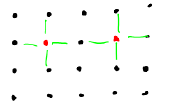
\includegraphics[width=0.3\textwidth]{\main/Images/image026.png}
    \caption{Square lattice with two flipped non-neighbouring spins (in red).\label{fig:two-flip-far}}
\end{figure}

Suppose $\sigma_i$ and $\sigma_j$ are \textbf{not neighbours}  - meaning that they are independent (\ref{fig:two-flip-far}). Then the change in the sums $A$ and $B$ will just be \textit{twice} that produced by flipping only one spin, and the exponential will be:
\begin{align}
    \mathcal{N}_{2,\mathrm{far}} = \exp\left[(2V -16)K + (V-4)h\right]
\end{align}
How many configurations $\{\bm{\sigma}\}$ generate such term? The first spin to flip $\sigma_i$ may be anyone of the $V$ spins in the system, but the second $\sigma_j$ cannot be in the same position, not in one of the $4$ neighbouring cells, leaving available only $V-5$ places. Thus, so far we have $V(V-5)$ configurations. Exchanging $\sigma_i$ and $\sigma_j$ will not alter anything - as they are both $-1$ - and so we need to divide by $2$ the previous total, leading to $V(V-5)/2$:
\begin{align*}
    Z = \mathcal{N}_0 + V \mathcal{N}_1 + \frac{V(V-5)}{2} \mathcal{N}_{2,\mathrm{far}} + \dots
\end{align*}
If the two flipped spins are instead \textbf{neighbours}, then $B$ will change the same (by $-4$), but for $A$ we need to account only $6$ changed interactions, and not $8$: one \textit{edge} is in common between the two spins, contributing with a $\sigma_i \sigma_j = (-1)(-1) = +1$, as if it was never changed, leaving $3$ affected edges for each spin (fig. \ref{fig:two-flip-close}).

\begin{figure}[H]
    \centering
    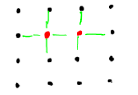
\includegraphics[width=0.3\textwidth]{\main/Images/image025.png}
    \caption{Square lattice with two flipped neighbouring spins (in red).\label{fig:two-flip-close}}
\end{figure}

So the new exponential term will be:
\begin{align*}
    \mathcal{N}_{2,\mathrm{close}} = \exp[(2V - 12)K + (V-4)h]
\end{align*}
The first spin can go in $V$ places, but the second one must be its neighbour, leaving only $4$ possibilities. Dividing by $2$ to account for their permutation leaves us with $2V$ configurations forming $\mathcal{N}_{2,\mathrm{close}}$:
\begin{align*}
    Z &= \mathcal{N}_0 + V \mathcal{N}_1 + \frac{V(V-5)}{2} \mathcal{N}_{2,\mathrm{far}} + 2V \mathcal{N}_{2,\mathrm{close}} + \dots =\\
    &= e^{2VK + hV} + V e^{(2V-8)K + (V-2)h} + \frac{V(V-5)}{2} e^{(2V-16)K + (V-4)h}  + 2V e^{(2V-12)K + (V-4)h} + \dots
\end{align*}
Note that substituting $\bm{\sigma} \leftrightarrow -\bm{\sigma}$ is equivalent to changing the sign of $h$. In fact, any term of the sum in (\ref{eqn:Z-again}) changes by:
\begin{align*}
    \exp\left(K \sum_{\langle x,y \rangle} \sigma_x \sigma_y + h \sum_x \sigma_x\right) \xrightarrow[\bm{\sigma} \leftrightarrow -\bm{\sigma}]{} \exp\left(K \sum_{\langle x,y \rangle}(\cancel{-}\sigma_x)(\cancel{-}\sigma_y) - h\sum_x \sigma_x\right)
\end{align*}
So, by changing the sign of $h$ in all the terms we already found, we can construct their \textit{reflections} - i.e. the ones starting from all spins \textit{down} and flipping \textit{up} $1$ or $2$ of them. Adding them to $Z$ we get:
\begin{align*}
    Z &= \hlc{SkyBlue}{e^{V(2K+h)}}\left[1+ V e^{-8K - 2h} + \frac{V(V-5)}{2} e^{-16K - 4h} + 2 V e^{-12K - 4h}  + O(e^{-16K - 6h}) \right] +\\
    &+\,\hlc{Yellow}{e^{V(2K-h)}}\left[1 + V e^{-8K + 2h} + \frac{V(V-5)}{2} e^{-16K + 4h} + 2 V e^{-12K + 4h} + O(e^{-16K + 6h})\right] 
\end{align*}
In fact, considering $3$ spin-flips leads to new terms of order $O(e^{-16K - 6h})$ (if they happen to be all neighbouring, as there are $8$ affected interactions), or higher (if they are further apart, for up to $12$ affected interactions).

\medskip

Starting with $h > 0$ and taking first the thermodynamic limit $V \to \infty$ and then $h \downarrow 0^+$ we note that only the first series of terms \textit{dominates}. In fact, for any $h > 0$:
\begin{align*}
    \lim_{V \to \infty} \frac{\hlc{Yellow}{e^{V(2K-h)}}}{\hlc{SkyBlue}{e^{V(2K+h)}}} = \lim_{V \to \infty} e^{-2h} = 0 \qquad \forall h > 0
\end{align*}

So in the thermodynamic limit we can ignore the terms in the second row. 
Taking the logarithm and dividing by $V$ we get the series expansion of the free energy:
\begin{align*}
    \frac{\ln Z}{V} = -\beta f(K,h) = 2K + h +\frac{1}{V} \ln \left[1+ V e^{-8K-2h} + \frac{V(V-5)}{2} e^{-16K - 4h} +2V e^{-12K - 4h} + \dots \right]   
\end{align*}
For $T \to 0$, $\beta \to \infty$, and so $K = \beta J \to \infty$, meaning that $e^{-K} \to 0$ and so we may expand in series the logarithm: 
\begin{align*}
    \ln (x) \approx x -\frac{x^2}{2} + O(x^3) 
\end{align*}
leading to:
\begin{align*}
    -\beta f(K,h) &= 2K+h + \underbrace{e^{-8K-2h} + \frac{\cancel{V}-5}{2} e^{-16K-4h} +2 e^{-12K-4h}}_{\text{First term}} \\
    &\quad\>-\cancel{\frac{1}{2V} (V e^{-8k-2h})^2 }+ O(e^{-16k-6h}) =\\
    &= 2 K +h + e^{-8K -2h} + 2 e^{-12K-4h} -\frac{5}{2}e^{-16K-4h} + O(e^{-16k - 6h}) 
\end{align*}

The spontaneous magnetization is then:
\begin{align}\nonumber
    m \underset{\substack{(\ref{eqn:magnetization})\\(\ref{eqn:break1})}}{=} \frac{1}{V} \pdv{\ln Z}{h} \Big|_{h=0} &= 1 -2 e^{-8K-2h}  -8e^{-12K-4h} + 10 e^{-16K-4h} + \dots \Big|_{h=0} =\\
    &= 1 - 2e^{-8K} -8 e^{-12K} + 10e^{-16K} + \dots \label{eqn:m-low}
\end{align}
and is plotted in fig. \ref{fig:m-expansion}.

\begin{figure}[H]
    \centering
    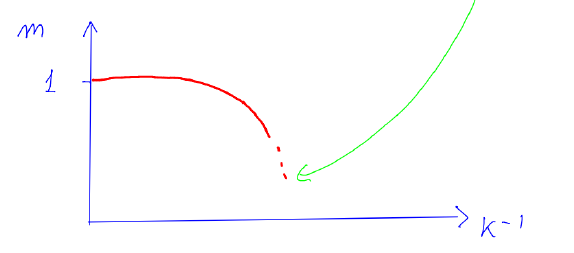
\includegraphics[width=0.7\textwidth]{\main/Images/image027.png}
    \caption{Plot of the spontaneous magnetization as function of temperature $T \propto K^{-1} = 1/(\beta J)$. For $T \to 0$ ($K \to \infty$) $m$ goes to $1$. From Onsager's exact solution we know that $m$ reaches $0$ at $T_c$, but this cannot be observed in this expansion, as the radius of convergence never includes $T_c$. \label{fig:m-expansion}}
\end{figure}

\begin{appr}\textbf{More terms}. For more terms of the expansion in (\ref{eqn:m-low}) see \cite{low-exp}. There also next nearest neighbours interactions are considered, with an interaction strength $J_2$ - so, to reconstruct our case, let $J_2 = 0$ and thus $y = e^{-4J_2 \beta} = 1$. So, formula (3) in \cite{low-exp} may be adapted as:
    \begin{align*}
        M(x) = 1-2x^2 y^2 + \sum_{m,n} a(m,n) x^m y^n \Big|_{y=1} \qquad x=e^{-4K}
    \end{align*}
    Borrowing coefficients from table $1$ in \cite{low-exp} we get:
    \begin{align*}
        M(K) = 1 - 2 e^{-8K} -8 e^{-12K} + (-8+ 18-24-20) e^{-16K} + \dots
    \end{align*}
    So the first coefficients in (\ref{eqn:m-low}) are correct, but the one for $e^{-16K}$ not. In fact, to refine it, we should also consider the case of $3$ and $4$ neighbouring flips, which add terms of the same order $e^{-16K}$, but are much more difficult to compute.

    \medskip

    Fortunately, there are more sophisticated methods for generating more terms, as can be seen in \cite{ising-low}
\end{appr}

\subsection{Correlation functions}
Until now we analysed the \textit{magnetization}, i.e. the average local spin alignment:
\begin{align*}
    m_x \equiv \langle \sigma_x \rangle
\end{align*} 
This can be interpreted as a \textbf{one-point} correlation function, measuring how much a spin $\sigma_x$ is \q{correlated} with itself.

\medskip

If we instead compare $\sigma_x$ with a \textit{different} spin $\sigma_y$, we get the \textbf{two-point} correlation function:
\begin{align}\label{eqn:two-point}
    G_{x,y}^{(2)} = \operatorname{Cov}[\sigma_x, \sigma_y] = \langle \sigma_x \sigma_y \rangle - \langle \sigma_x \rangle \langle \sigma_y \rangle
\end{align}   
If $\sigma_x$ and $\sigma_y$ are independent, then immediately $\langle \sigma_x \sigma_y \rangle = \langle \sigma_x \rangle \langle \sigma_y \rangle$, and so $G_{x,y}^{(2)} = 0$. In general, however, the converse is not true: if the two-point correlation is $0$, the two spin may still be interacting.

\medskip

Consider each spin interacting with a local field $h_x$ in the Ising Model. The partition function is then:
\begin{align*}
    Z(\bm{h}) = \sum_{\{\bm{\sigma}\}} \exp\left(-\beta \mathcal{H}(\bm{\sigma}) + \sum_x h_x \sigma_x \right) \equiv e^{-\beta F(\bm{h})}
\end{align*}
with $F$ being the corresponding \textbf{free energy}. This is a generalization of the case (\ref{eqn:Z-again}), where $h_x \equiv h$ for all spins. Being able to \textit{vary} the local field experienced by a single spin allows us to write correlation functions as derivatives of $Z$. 

\medskip

For the one-point correlation we get the same formula previously found in (\ref{eqn:magnetization}):
\begin{align}\label{eqn:mag2}
    m_x = -\pdv{h_x} (\beta F(\bm{h}))
\end{align}
On the other hand, for the two point correlation we get:
\begin{align}\label{eqn:G2}
    G_{xy}^{(2)} = -\pdv[2]{}{h_x}{h_y} (\beta F(\bm{h})) = \langle (\sigma_x - \langle \sigma_x \rangle) (\sigma_y - \langle \sigma_y \rangle)\rangle \underset{(\ref{eqn:mag2})}{=}  \pdv{m_y}{h_y}
\end{align}
Similarly, for a $3$-point correlation:
\begin{align*}
    G_{xyz}^{(3)} = -\frac{\partial^3}{\partial h_x \partial h_y \partial h_z} (\beta F(\bm{h})) = \langle (\sigma_x - \langle \sigma_x \rangle) (\sigma_y - \langle \sigma_y \rangle) (\sigma_z - \langle \sigma_z \rangle) \rangle 
\end{align*}
and in general:
\begin{align*}
    G_{x_1,\dots,x_n}^{(n)} = - \frac{\partial^n}{\partial h_{x_1}\cdots \partial h_{x_n}}  (\beta F)
\end{align*}

We define the \textbf{susceptibility}\marginpar{Susceptibility $\chi$}\index{Susceptibility} as the derivative of the magnetization $m$ with respect to the field $h$ (when $h_x \equiv h$ $\forall x$):
\begin{align*}
    \chi &\equiv \pdv{m}{h}
\end{align*}
Inserting the definition of the magnetization (\ref{eqn:magnetization}) and computing the averages leads to:
\vspace{-2em}
\begin{align*}
    \chi &\equiv \pdv{m}{h} = \pdv{h} \langle \sum_x \sigma_x \rangle \frac{1}{V} = \frac{1}{V} \sum_x \pdv{h} \langle \sigma_x \rangle  = \frac{1}{V} \sum_x \pdv{h}
    \frac{\displaystyle \overbrace{\sum_{\{\bm{\sigma}\}} \sigma_x \exp\left(- \beta \mathcal{H}(\bm{\sigma}) + \sum_y h \sigma_y \right)}^{\mathclap{\mathrm{Num}}} }{\underbrace{Z(\bm{h})}_{\mathrm{Den}} } = \\
    &= \frac{1}{V} \sum_x 
    \frac{\displaystyle \overbrace{\sum_{\{\bm{\sigma}\}} \exp\left(-\beta \mathcal{H}(\bm{\sigma}) + \sum_y h \sigma_y\right) \sum_y \sigma_y}^{(\partial_h \mathrm{Num}) / \mathrm{Den}  } }
         {Z(\bm{h})} +\\
    &-\frac{1}{V}\sum_x \underbrace{\frac{\displaystyle 
    \sum_{\{\bm{\sigma}\}} \sigma_x \exp\left(- \beta \mathcal{H}(\bm{\sigma}) + \sum_y h \sigma_y\right)}{Z(\bm{h})}\cdot \frac{\displaystyle \sum_{\{\bm{\sigma}\}} \exp\left(-\beta \mathcal{H}(\bm{\sigma}) + \sum_y h \sigma_y \right) \sum_y \sigma_y}{Z(\bm{h})} }_{-(\mathrm{Num} \,\partial_h \mathrm{Den}) / \mathrm{Den}^2 } =\\
    &= \frac{1}{V}\left[\langle \sum_{x,y} \sigma_x \sigma_y \rangle - \langle \sum_x \sigma_x \rangle \langle \sum_y \sigma_y \rangle\right] 
\end{align*}
So, rewriting the last step result in terms of (\ref{eqn:G2}) we get:\marginpar{Fluctuation dissipation theorem}\index{Theorem!Fluctuation dissipation}
\begin{align*}
    \chi = \sum_x G_{x,y}
\end{align*}
This the \textbf{fluctuation dissipation theorem}. In other words, the \q{total} \textit{correlation} between one spin $\sigma_x$ and every other spin $\sigma_y$ is equal to the \q{responsivity} of $m_x$ to a change in $h$, i.e. how much the alignment of $\sigma_x$ varies when the external field $b = h/\beta$ is adjusted.
 
\medskip

$\mathcal{H}$ is translational invariant if it does not change when \textit{translating} spins: 
\begin{align*}
    \mathcal{H}(\bm{\sigma}) = H(\bm{\sigma}')
\end{align*}
with $\sigma_x' = \sigma_{x+x_0}$ for any $x$ and $x_0$ fixed.

In this case, as we previously noted, the magnetization is constant: $m = \langle \sigma_x \rangle$, and the two-point correlation depends only on the distance between the two spins: $\langle \sigma_x \sigma_y \rangle = \langle \sigma_{x-y} \sigma_0 \rangle$.

\medskip

Finally, we compute the Legendre transform $\Gamma(m)$ of $\beta F$ with respect to $h$:
\begin{align*}
    \Gamma(\bm{m}) = \beta F(\bm{j}) + \sum_x h_x m_x
\end{align*}
where the $\{h_x\}$ have been calculated as a function of the local magnetizations $\{m_x\}$ by inverting (\ref{eqn:mag2}). By property of the Legendre transform:
\begin{align*}
    \pdv{\Gamma}{m_x} = h_x
\end{align*}
Differentiating both sides with respect to $h_y$ leads to:
\begin{align*}
    \delta_{xy} = \sum_z \pdv[2]{\Gamma}{m_x m_z} \pdv{m_z}{h_y} \underset{(\ref{eqn:two-point})}{=} \sum_z \pdv[2]{\Gamma}{m_x}{m_z} G_{zy}
\end{align*}
Thus $\pdv[2]{\Gamma}{m_x}{m_y}$ is the inverse of the two-point correlation function $G_{xy}$. %Check this last part.


\begin{exo}[Ising Model]
    Consider a $1$-dimensional Ising Model with nearest-neighbour ferromagnetic interaction in an external uniform field with energy function given by:
    \begin{align*}
        \mathcal{H}(\bm{\sigma}) = -J \sum_{x=1}^N \sigma_x \sigma_{x+1} - B \sum_{x=1}^N \sigma_x \qquad J > 0
    \end{align*}    
    where periodic boundary conditions are used, i.e. $\sigma_{N+1} \equiv \sigma_1$. Define $K = \beta J$ and $\beta B = h$.
    
    \medskip
    
    \textbf{Part A}. Using the transfer matrix $T(\sigma, \sigma') = \exp(K \sigma \sigma' + h (\sigma + \sigma')/2)$ and its spectral decomposition, determine:
    \begin{enumerate}
        \item The \textbf{partition function} $Z(K,h)$
        \item The \textbf{free energy} per node in the thermodynamic limit and its plot for $h=0$ versus $1/K$
        \item The \textbf{entropy} per node in the thermodynamic limit and its plot for $h=0$ versus $1/K$
        \item The \textbf{mean energy} per node in the thermodynamic limit and its plot for $h=0$ versus $1/K$
        \item The \textbf{specific heat} per node in the thermodynamic limit and its plot for $h=0$ versus $1/K$
        \item The \textbf{average magnetization} at $x$, $\langle \sigma_x \rangle$, in the thermodynamic limit and its plot for $h=0, 0.1, 0.2, 0.5, 1$ versus $1/K$ and for $K=1$ versus $h$ in the range $(-5,5)$
        \item The \textbf{two-point correlation function} $\langle \sigma_x \sigma_{x+y} \rangle$ in the thermodynamic limit and its plot for $h=0$ and $K=1$ versus $y$.
    \end{enumerate}

    \textbf{Part B}. Consider the same model with \textbf{open} boundary conditions (node $1$ is linked only to node $2$, and node $N$ only to node $N-1$):
    \begin{align*}
        \mathcal{H}(\bm{\sigma}) = -J \sum_{x=1}^{N-1} \sigma_x \sigma_{x+1} - B \sum_{x=1}^N \sigma_x
    \end{align*}   
    Show that the partition function for this case can be formally written as:
    \begin{align*}
        Z(K,h) = \bm{v}^T \textbf{T}^N \bm{v} \equiv \sum_{\substack{\sigma_1 = \pm 1\\ \sigma_N = \pm 1}} v(\sigma_1) \textbf{T}^N(\sigma_1, \sigma_N) v(\sigma_N)  
    \end{align*}
    where $v(\sigma) = e^{h \sigma /2}$. Show that the free energy per node in the thermodynamic limit is the same as above.
    
    \medskip

    \textbf{Part C}. Same as in part $B$ with fixed boundary conditions $\sigma_1 = 1 = \sigma_2$, and $v(\sigma) = e^{h/2}$ for both $\sigma=\pm 1$.
    
    \medskip

    \textbf{Part D}. How would you try to solve the Ising model in $1$-dimension with nearest neighbour and next-to-nearest neighbour interaction and periodic boundary condition ($\sigma_{N+1} = \sigma_1$ and $\sigma_{N+2} = \sigma_2$):
    \begin{align*}
        \mathcal{H}(\bm{\sigma}) = -\sum_{x=1}^N (J_1 \sigma_x \sigma_{x+1} + J_2 \sigma_x \sigma_{x+2}) - B \sum_{x=1}^N \sigma_x
    \end{align*} 

    \medskip

    \textbf{Solution}. WIP %TO DO
     
\end{exo}

%Variational methods move to following day.
\end{document}
